\documentclass{article}[a4paper]

\usepackage[czech]{babel}
\usepackage[T1]{fontenc}
\usepackage{geometry}
\usepackage{graphicx}
\usepackage[pdfusetitle]{hyperref}

\title{Implementační dokumentace k~2. úloze do IPP 2023/2024}
\author{Milan Vodák}

\begin{document}
    \begin{center}
        {\Large Implementační dokumentace k~2. úloze do IPP 2023/2024}

        Jméno a příjmení: Milan Vodák

        Login: xvodak07
    \end{center}

    \section{Diagram tříd}

    \begin{center}
        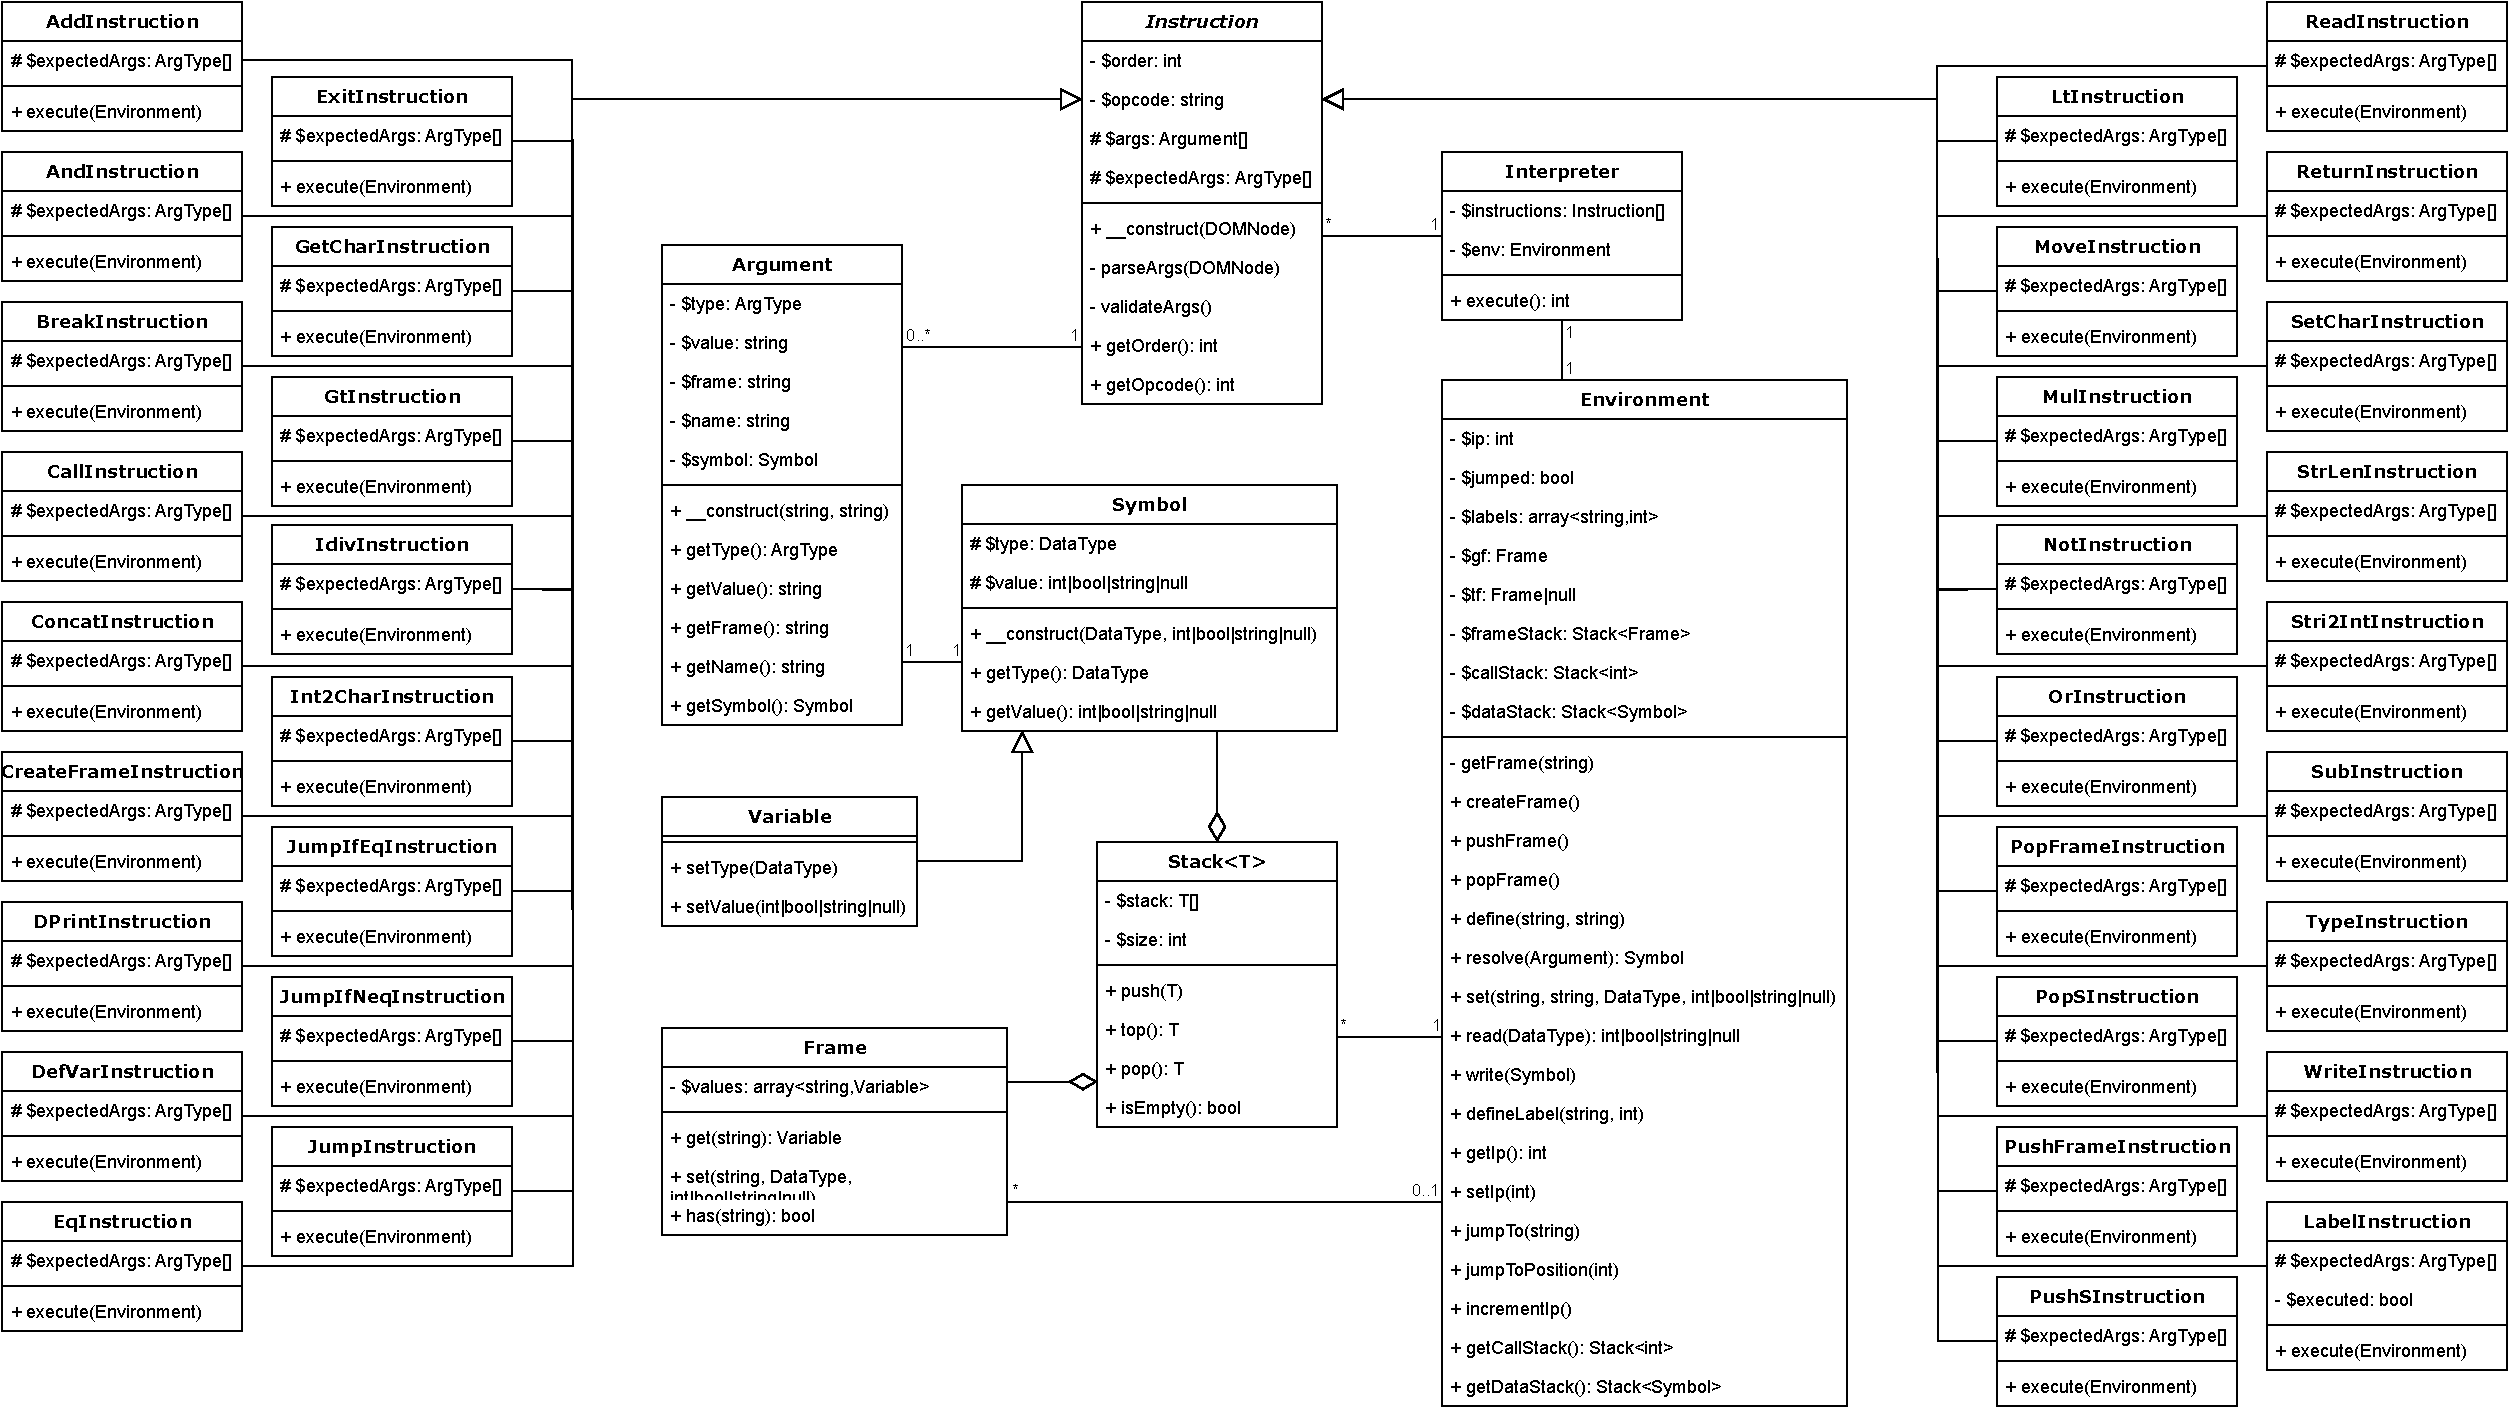
\includegraphics[width=\textwidth]{class-diagram.pdf}
    \end{center}

    \section{Popis částí}

    \subsection{\texttt{Interpreter}}

    Třída \texttt{Interpreter} implementuje metodu \texttt{execute()}, která je vstupním bodem celého interpretu.
    Nejprve provádí zpracování a validaci vstupního XML souboru a z~dat vytváří instance instrukcí, které si ukládá do pole.
    Následně provede jeden průchod programem, při němž spouští pouze instrukce \texttt{LABEL} tak, aby před skutečným začátkem interpretace byla definována všechna návěští.
    Nakonec nastaví čítač instrukcí zpět na začátek a s~jeho použitím vykonává jednotlivé instrukce.

    \subsection{\texttt{Environment}}

    Třída \texttt{Environment} popisuje běhové prostředí a aktuální stav interpretu (jinými slovy kontext interpretace).
    Prostředí obsahuje zásobník rámců, globální a dočasný rámec, zásobník volání i datový zásobník.
    Navíc uchovává definovaná návěští a číslo aktuálně prováděné instrukce (\emph{instruction pointer}).
    Třída poskytuje metody pro manipulaci s~rámci, proměnnými a návěštími a pro provádění skoků.
    Prostřednictvím nich komunikují prováděné instrukce s~běhovým prostředím.

    Metody \texttt{jumpTo()} a \texttt{jumpToPosition()} umožňují provést skok na návěští, resp. konkrétní pozici úpravou instruction pointeru.
    Metoda \texttt{define()} slouží k~definici nových proměnných v~konkrétním paměťovém rámci a metoda \texttt{defineLabel()} k~definici návěští.
    Prostřednictvím metody \texttt{set()} je možné nastavit hodnotu proměnné podle názvu a rámce.
    Metoda \texttt{resolve()} podle daného argumentu vyhledá a vrátí proměnnou, nebo v~případě, že argument není proměnná, vrátí odpovídající symbol (viz Sekce \ref{sec:symbol}).

    \subsection{\texttt{Frame}}

    Paměťový rámec sestává z~asociativního pole proměnných, identifikovaných jejich názvem, a z~metod sloužících k~nalezení a nastavení hodnoty.

    \subsection{\texttt{Instruction}}
    \label{sec:instruction}

    Abstraktní třída \texttt{Instruction} je nadtřídou všech instrukcí z~instrukční sady a slouží jako jejich vzor.
    Atributy instrukcí jsou pořadí, operační kód, očekávané typy argumentů a pole obsahující skutečně načtené argumenty.
    Konstruktor, který je implementovaný pouze v~nadtřídě, provádí převod XML uzlu na instanci instrukce a jeho potomků na argumenty.
    Dále třída obsahuje implementace metod \texttt{parseArgs()} a \texttt{validateArgs()}, které zajišťují zpracování a validaci těchto argumentů.
    Nejdůležitější metoda, \texttt{execute()}, sloužící k~vykonání instrukce, musí být implementována v~každé podtřídě.

    \subsection{Instrukční sada}

    Každý typ instrukce, podporovaný interpretem, je reprezentován podtřídou třídy \texttt{Instruction} (viz Sekce \ref{sec:instruction}) ve jmenném prostoru \texttt{IPP\textbackslash Student\textbackslash Instruction}, přičemž každá konkrétní instrukce implementuje abstraktní metodu \texttt{execute()}.
    Také může redefinovat pole \texttt{expectedArgs}, které obsahuje typy argumentů, jež instrukce očekává.

    \subsection{\texttt{Argument}}

    Argument instrukce má typ vyjádřený výčtovým typem \texttt{ArgType} a obsahuje řetězec s~hodnotou přečtenou ze vstupu, objekt třídy \texttt{Symbol} (viz Sekce \ref{sec:symbol}) reprezentující
    konstantu, návěští nebo typ a atributy \texttt{name} a \texttt{frame}, které v~případě, že argument je proměnná, obsahují řetězec s~jejím rámcem, resp. názvem.

    \subsection{\texttt{Symbol}}
    \label{sec:symbol}

    Symbolem se rozumí konkrétní hodnota v~programu -- konstanta, návěští nebo typ -- případně proměnná reprezentovaná podtřídou.
    Instance symbolu je vytvořena při instanciaci argumentu, který není proměnnou, nebo při ukládání hodnot na datový zásobník.

    Symbol má datový typ určený výčtovým typem \texttt{DataType} a hodnotu, na niž se v~závislosti na tomto typu nahlíží jako na \texttt{int}, \texttt{bool}, \texttt{string} nebo \texttt{null}.

    \subsection{\texttt{Variable}}

    Proměnná je podtřídou třídy \texttt{Symbol} (viz Sekce \ref{sec:symbol}) a oproti běžnému symbolu má navíc možnost prostřednictvím metod měnit svůj typ a hodnotu.

    \subsection{\texttt{Stack}}

    Třída \texttt{Stack} je běžnou implementací zásobníku.
    Je to generická třída typovaná s~využitím standardu PHPDoc, díky čemuž může zásobník obsahovat hodnoty libovolného určeného typu a jediná třída je tak
    použita nejen jako zásobník rámců (typ \texttt{Frame}), ale i jako zásobník volání (typ \texttt{int}) a datový zásobník (typ \texttt{Symbol}).

    \subsection{Výjimky}

    Výjimky definované ve jmenném prostoru \texttt{IPP\textbackslash Student\textbackslash Exception} jsou přímými potomky třídy \texttt{IPPException}.
    Každá z~nich odpovídá jinému návratovému kódu a ty, u~nichž je to vhodné, navíc přijímají jako parametr instanci instrukce, při jejímž provádění chyba nastala, a zmiňují ji v~chybové hlášce.
    Z~důvodu přehlednosti jsou výjimky vynechány v~diagramu tříd.
\end{document}
